\section{Imagination Augmented Agent (I2A)} 
\label{sec:i2a} 
 
In the paper "Imagination-augmented agents for deep reinforcement learning" Weber et al. \cite{I2A} combines the advantages of model free and model based reinforcement learning to get an agent which is robost against model imperfections but is able to use the advantages of model based agents.\\ 
 
To do this they train a model of the environment for internal simulations. 
Imagine the future and learn to do better actions based on the imagined future.\\ 
 
Figure \ref{fig:i2a_architecture} shows the network architecture of the imagination-augmented agent. In the following the parts of the architecture will be explined 
 
\begin{figure}[H] 
  \centering 
   
  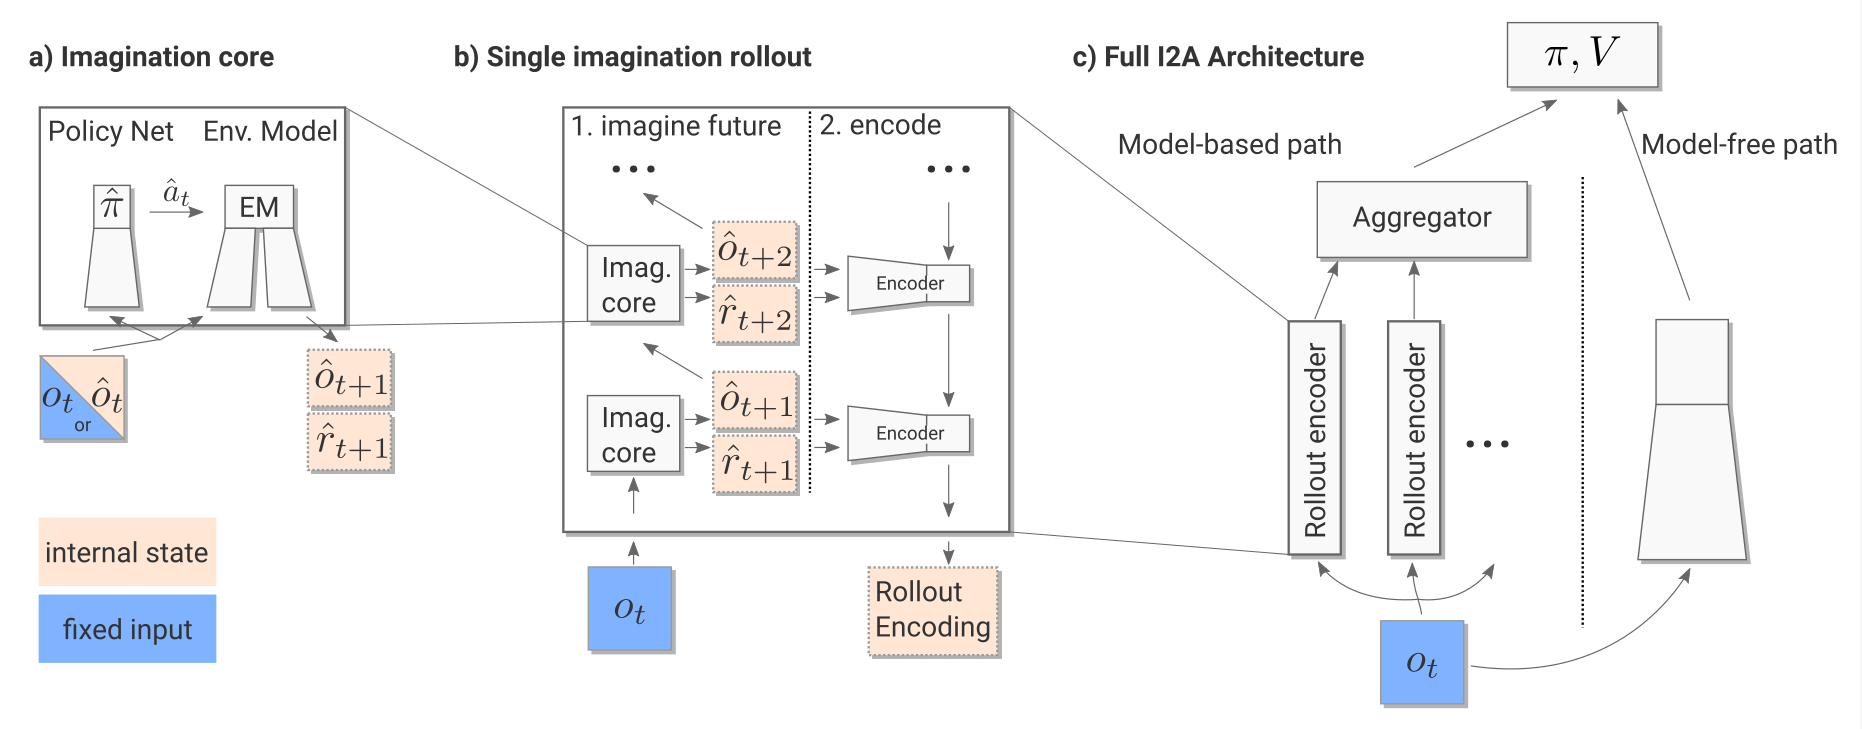
\includegraphics[width=\columnwidth]{./Images/i2a_architecture.png} 
  \caption{Network architecture for deep reinforcement learning which combines model free and model based reinforcement learning} 
  \label{fig:i2a_architecture} 
\end{figure} 
 
 
 
Imagination Core 
 
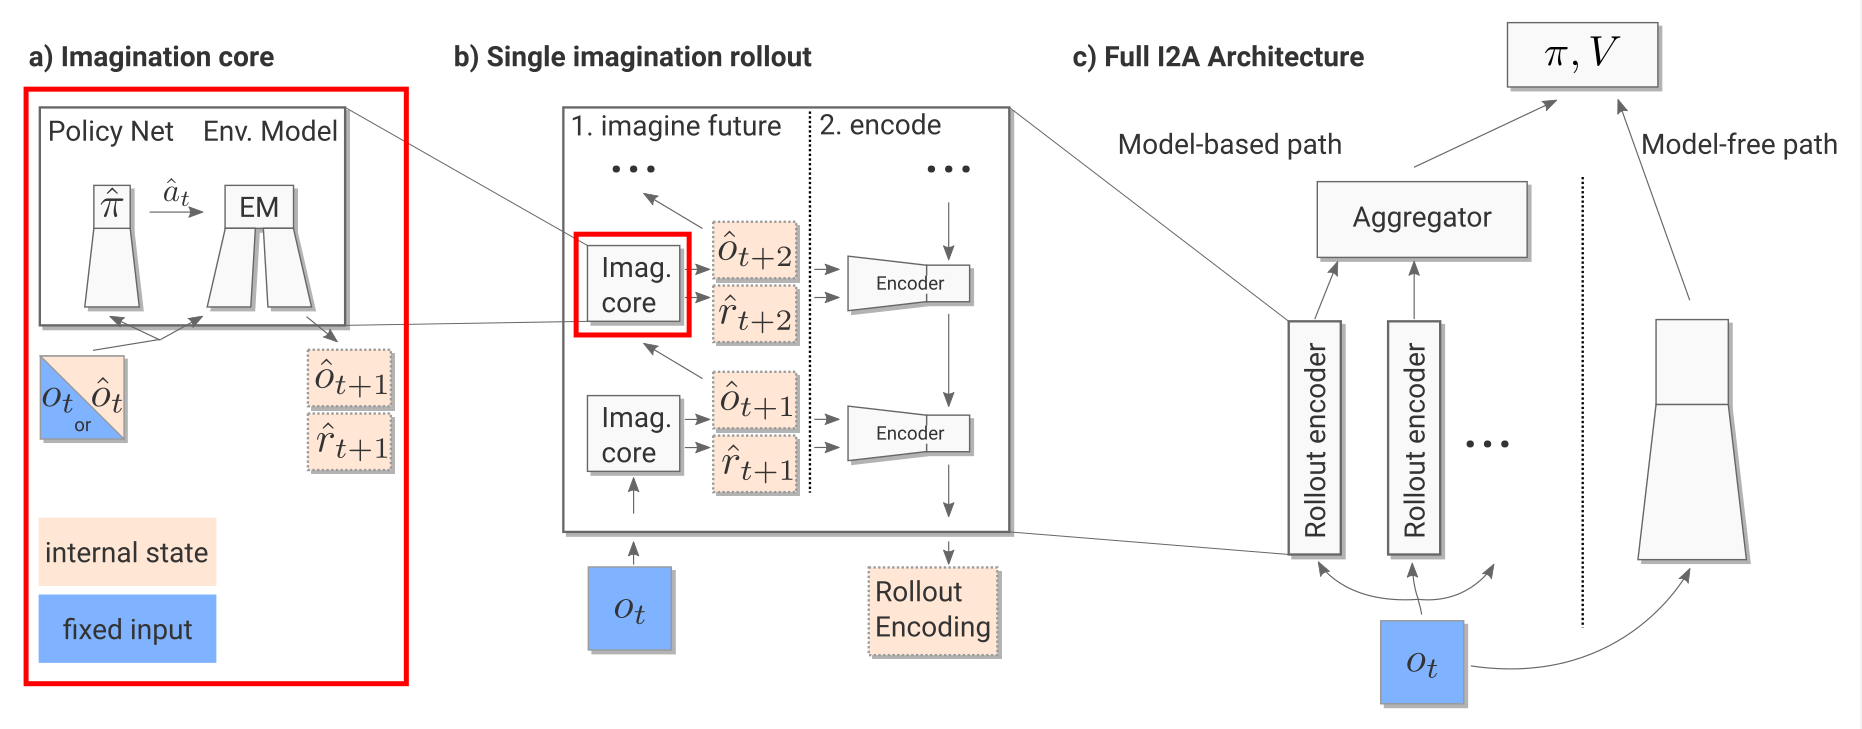
\includegraphics[width=\columnwidth]{./Images/i2a_all_imagination_core.png}% 
 
Imagine the next observation $\hat{o}_{t+i+1}$ and next reward $\hat{r}_{t+i+1}$ given observation $\hat{o}_{t+i}$ for n rollouts where $i = 0, ..., n$ 
%$\hat{}$ 
 
 
Rollout Policy Network $\hat{\pi}$ 
 
Rollout policy network $\hat{\pi}$ decides the next action $\hat{a}_t$ 
Distillation loss\\ 
Make $\hat{\pi}$ (rollout policy) and $\pi$ (i2a policy) similar\\ 
   
    %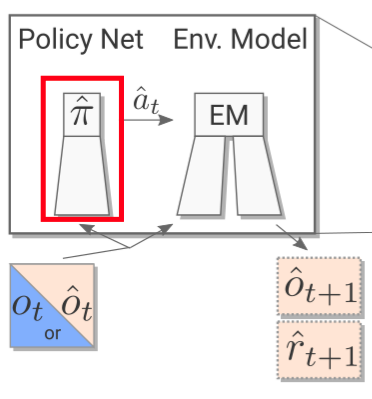
\includegraphics[height=0.35\textheight]{./Images/policy_net.png}% 
 
Cross Entropy between $\pi$ and $\hat{\pi}$\\ 
  \begin{equation} 
    l_{dist}(\pi, \hat{\pi})(o_t) = \lambda_{dist} \sum_a \pi(a | o_t) log \hat{\pi}(a|o_t) 
  \end{equation} 
     
 
 
Environment Model (EM) 
 
$o_t$: initial observation 
 $\hat{o}_t$: predicted observation 
 $\hat{r}_t$: predicted reward 
Given observation $o_t$ or $\hat{o}_t$ and action $\hat{a}_t$ predict (imagine) the next observation $\hat{o}_{t+1}$ and next reward $\hat{r}_{t+1}$  
   
  %\begin{center} 
    %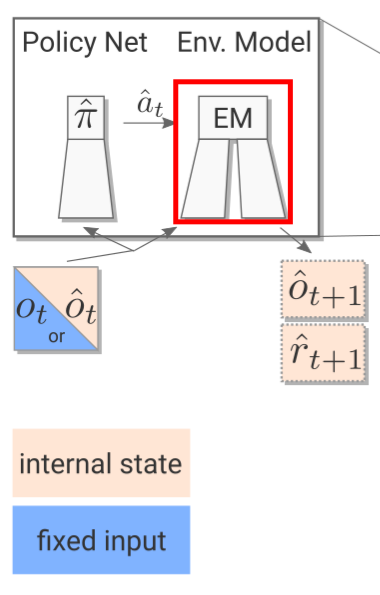
\includegraphics[height=0.5\textheight]{./Images/environment_model.png}% 
  %\end{center} 
 
 
Environment Model Architecture 
 
 Input:\\ 
    -- Stack of last 3 observations\\ 
    -- Action as one hot vector\\ 
Trained with paris of $(o_t, a_t) \rightarrow (o_{t+1}, r_{t+1})$ generated from a pretrained model-free advantage-actor-critic policy 
   
  %\begin{center} 
    %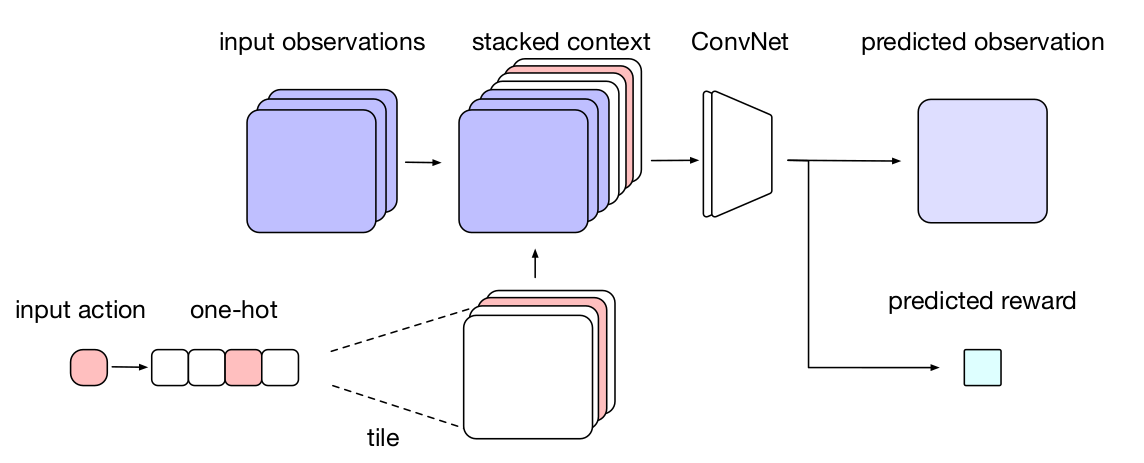
\includegraphics[width=\columnwidth]{./Images/environment_model_architecture.png}% 
  %\end{center} 
 
 
    Environment Model Training 
 
Maximize the log likelihood of the probability $\mathnormal{p(o_t | a_{t-1}, o_{t-1})}$ 
Image can be seen as Bernoulli distribution 
 
  \begin{equation} 
   p(o_t | a_{t-1}, o_{t-1}) = x^y (1-x)^{1-y} 
  \end{equation} 
   
  $\mathnormal{log p(o_t | a_{t-1}, o_{t-1})}$ equals to Binary Cross Entropy loss 
   
\begin{equation} 
  \mathnormal{ 
  env_{loss}(x, y) = \frac{1}{N} \sum y_n log x_n + (1-y_n) log(1- x_n) 
  %env_{loss} = Binary Cross Entropy(predicted\_image, true\_images) 
  } 
  \end{equation} 
 
 
 
 
I2A Architecture - Imagination Rollout 
 
 
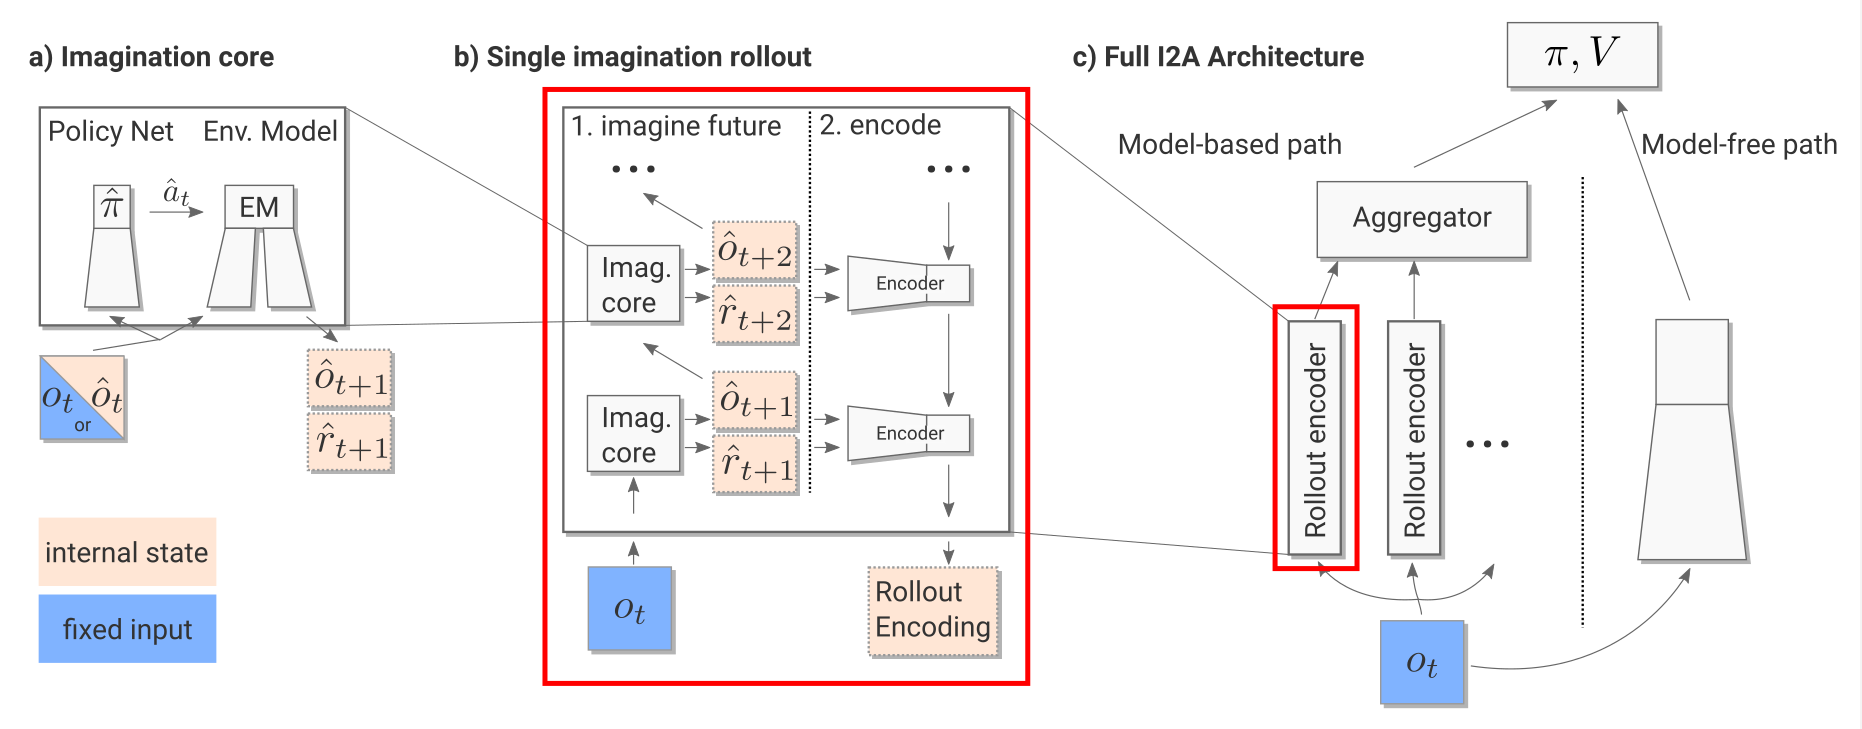
\includegraphics[width=\columnwidth]{./Images/i2a_all_imagination_rollout.png}% 
 
The imagination core imagines trajectories of features $f = (\hat{o}, \hat{r})$\\ 
The rollout encoder encode these trajectories     
 
 
 
I2A Architecture - Imagination Future 
 
Input:\\ 
    observation $o_t$ \\ 
    (1 MiniPacman frame)\\ 
    start action $a$ 
Output:\\ 
    n imagined trajectories ($\hat{o}_{t+i}, \hat{r}_{t+i}$ for $i = 0, ..., n$) 
     $\hat{} \hspace{2mm} \rightarrow$ internal state 
   
  %\begin{center} 
    %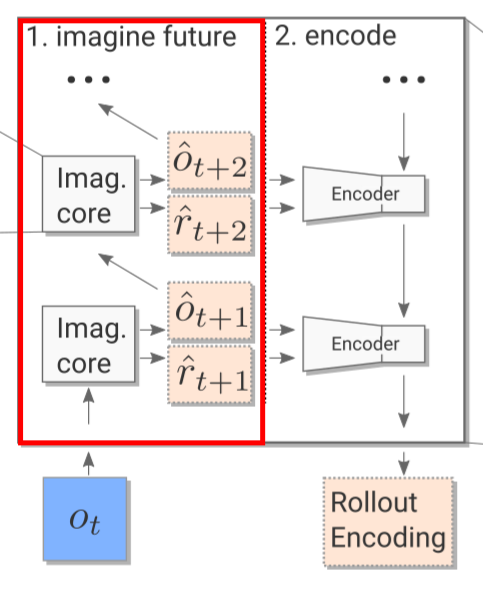
\includegraphics[height=.5\textheight]{./Images/imagine_future.png}% 
  %\end{center} 
 
I2A Architecture - Encoder 
 
     CNN Network followed by an LSTM Network 
    CNN Network:\\ 
    Encode observation and reward $\hat{o}_{t+i}, \hat{r}_{t+i}$ 
    LSTM Network:\\ 
    Learns long-term dependencies 
    %\item Learns useful information from the rollout trajectories 
   
  \begin{center} 
    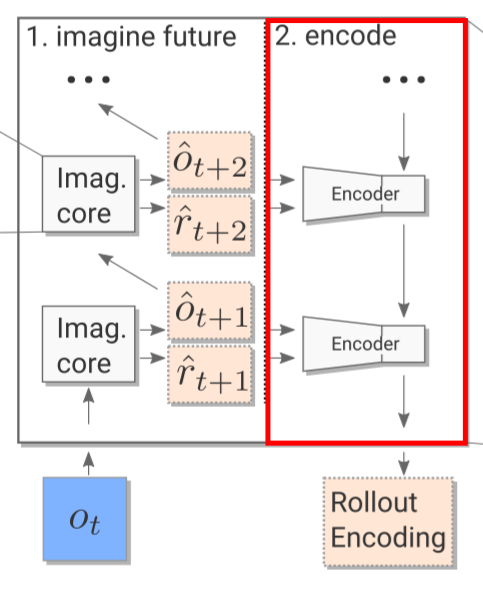
\includegraphics[height=.5\textheight]{./Images/encoder.png}% 
  \end{center} 
 
 
 
I2A Architecture - Model Based Path 
 
 
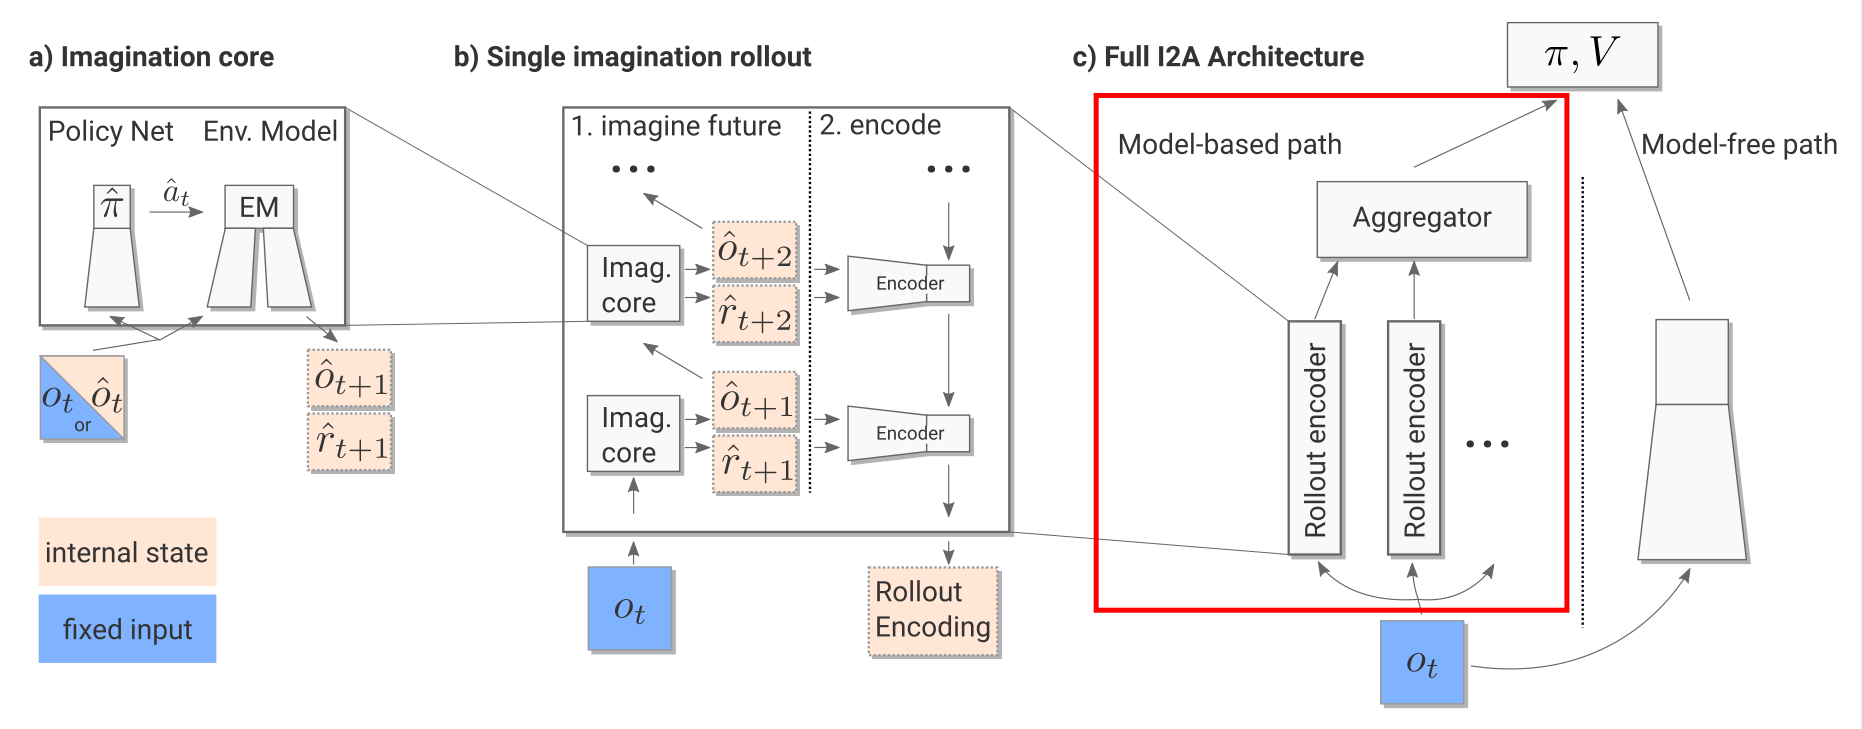
\includegraphics[width=\columnwidth]{./Images/i2a_all_model_based_path.png}% 
 
%For each action $a$ the agent can take do a imagination rollout  
% the future based on a model of the environment and use this information for decision making 
 
 
I2A Architecture - Model Based Path 
 
 
       For each action $a$ the agent can take, do a imagination rollout  
    %For each action the agent can take,  
    %imagine the future% and learn relevent information that can happen 
     Aggregator: \\ 
    Concatinate all action rollouts 
   
  %\begin{center} 
    %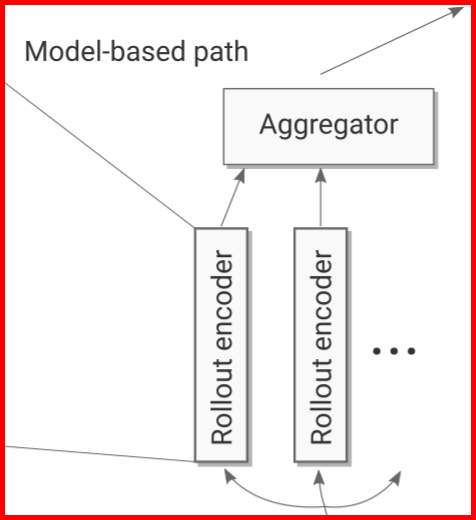
\includegraphics[height=.5\textheight]{./Images/i2a_model_based.png}% 
  %\end{center} 
 
 
 
I2A Architecture - Model Free Path 
 
 
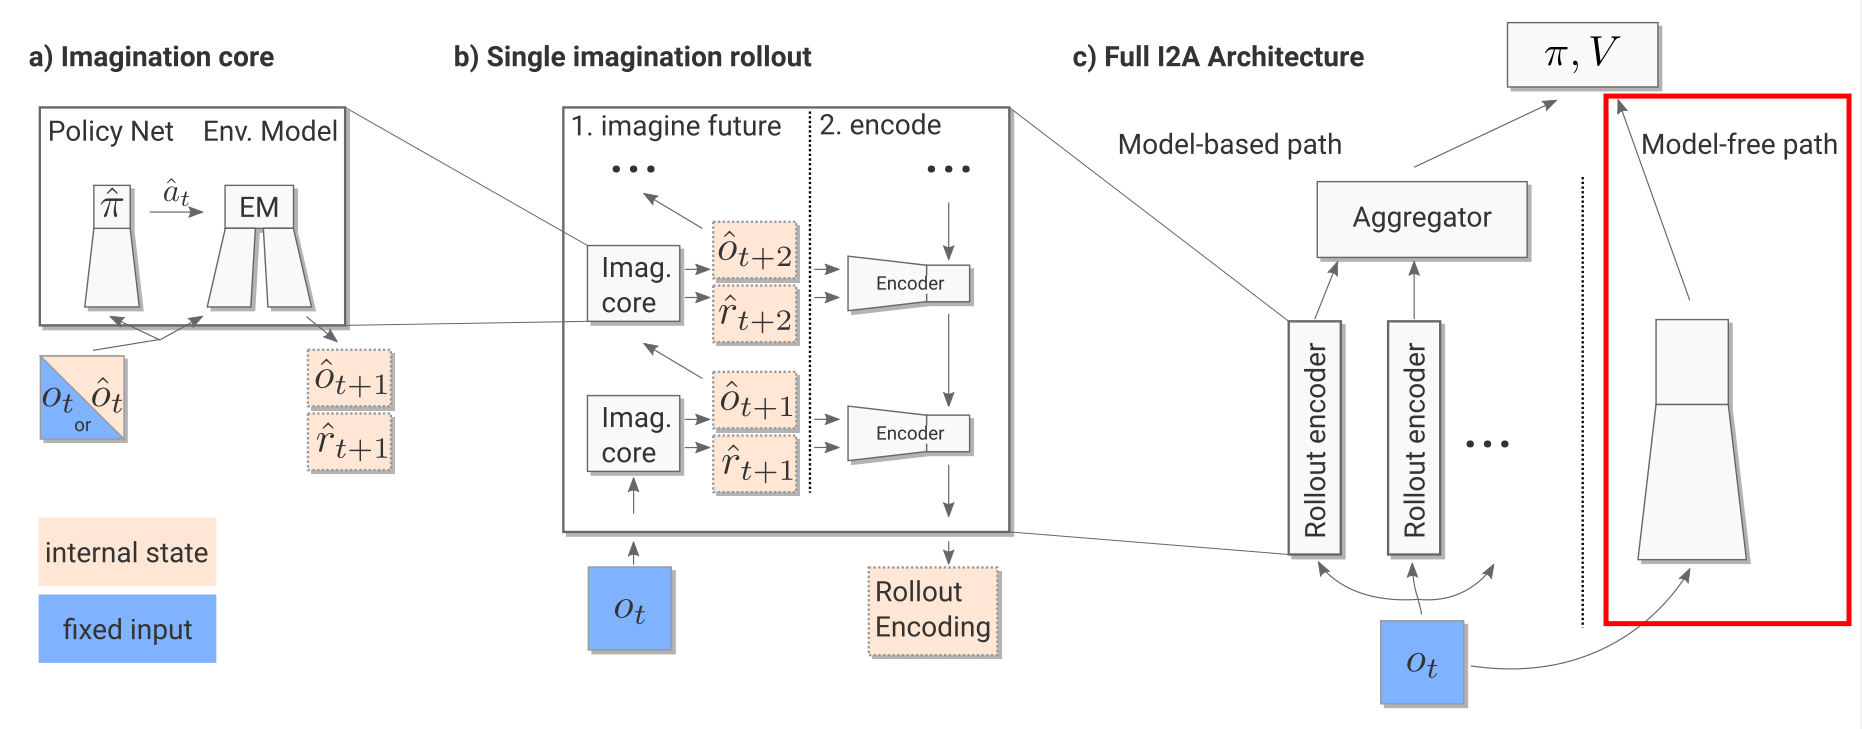
\includegraphics[width=\columnwidth]{./Images/i2a_all_model_free_path.png}% 
 
CNN Layers followed by Fully Connected Layers 
 
 
 
I2A Training 
Input:\\ 
    Observation $o_t$ 
     Output:\\ 
    Policy $\pi$ and value function $V$ 
     Train with Advantage-Actor-Critic (A2C) 
   
  \begin{center} 
    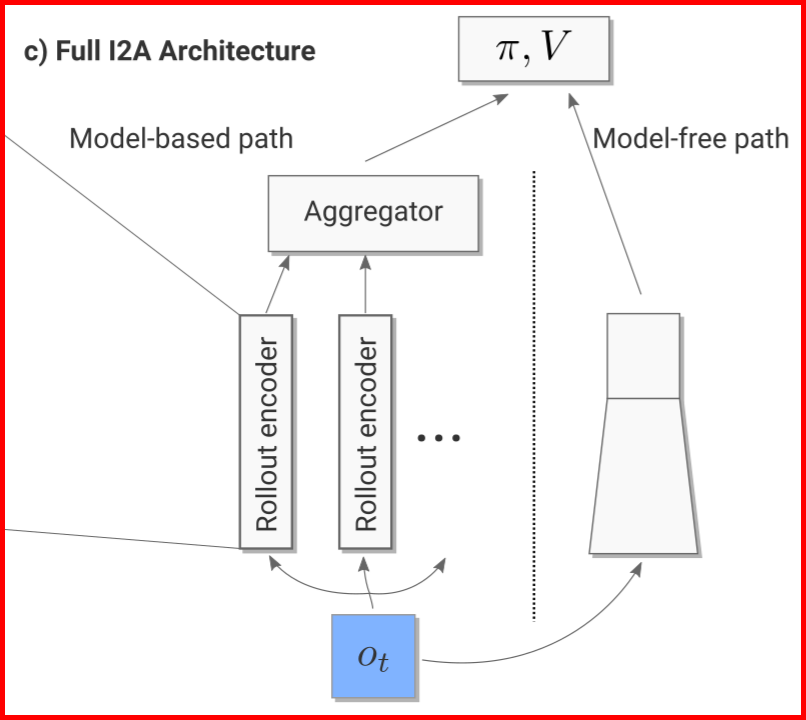
\includegraphics[width=\columnwidth]{./Images/i2a_a2c.png}% 
  \end{center} 
